\chapter{Registre de risques}

Les risques sont les probabilités que des événements indésirables surviennent, ayant des conséquences néfastes sur l'avancement du projet ou sur le produit final.
Il est important d'identifier les risques afin de leur faire face et de les éviter du mieux possible.
Un registre de risques permet justement d'énumérer les différents risques et de leur associer une stratégie de réduction du risque et un responsable.
Chaque risque a une probabilité d'occurrence, des conséquences possibles et des coûts en performances, ainsi qu'un niveau de priorité reflétant l'importance globale du risque.

\begin{figure}
  \centering
  \caption{Registre de risques}
  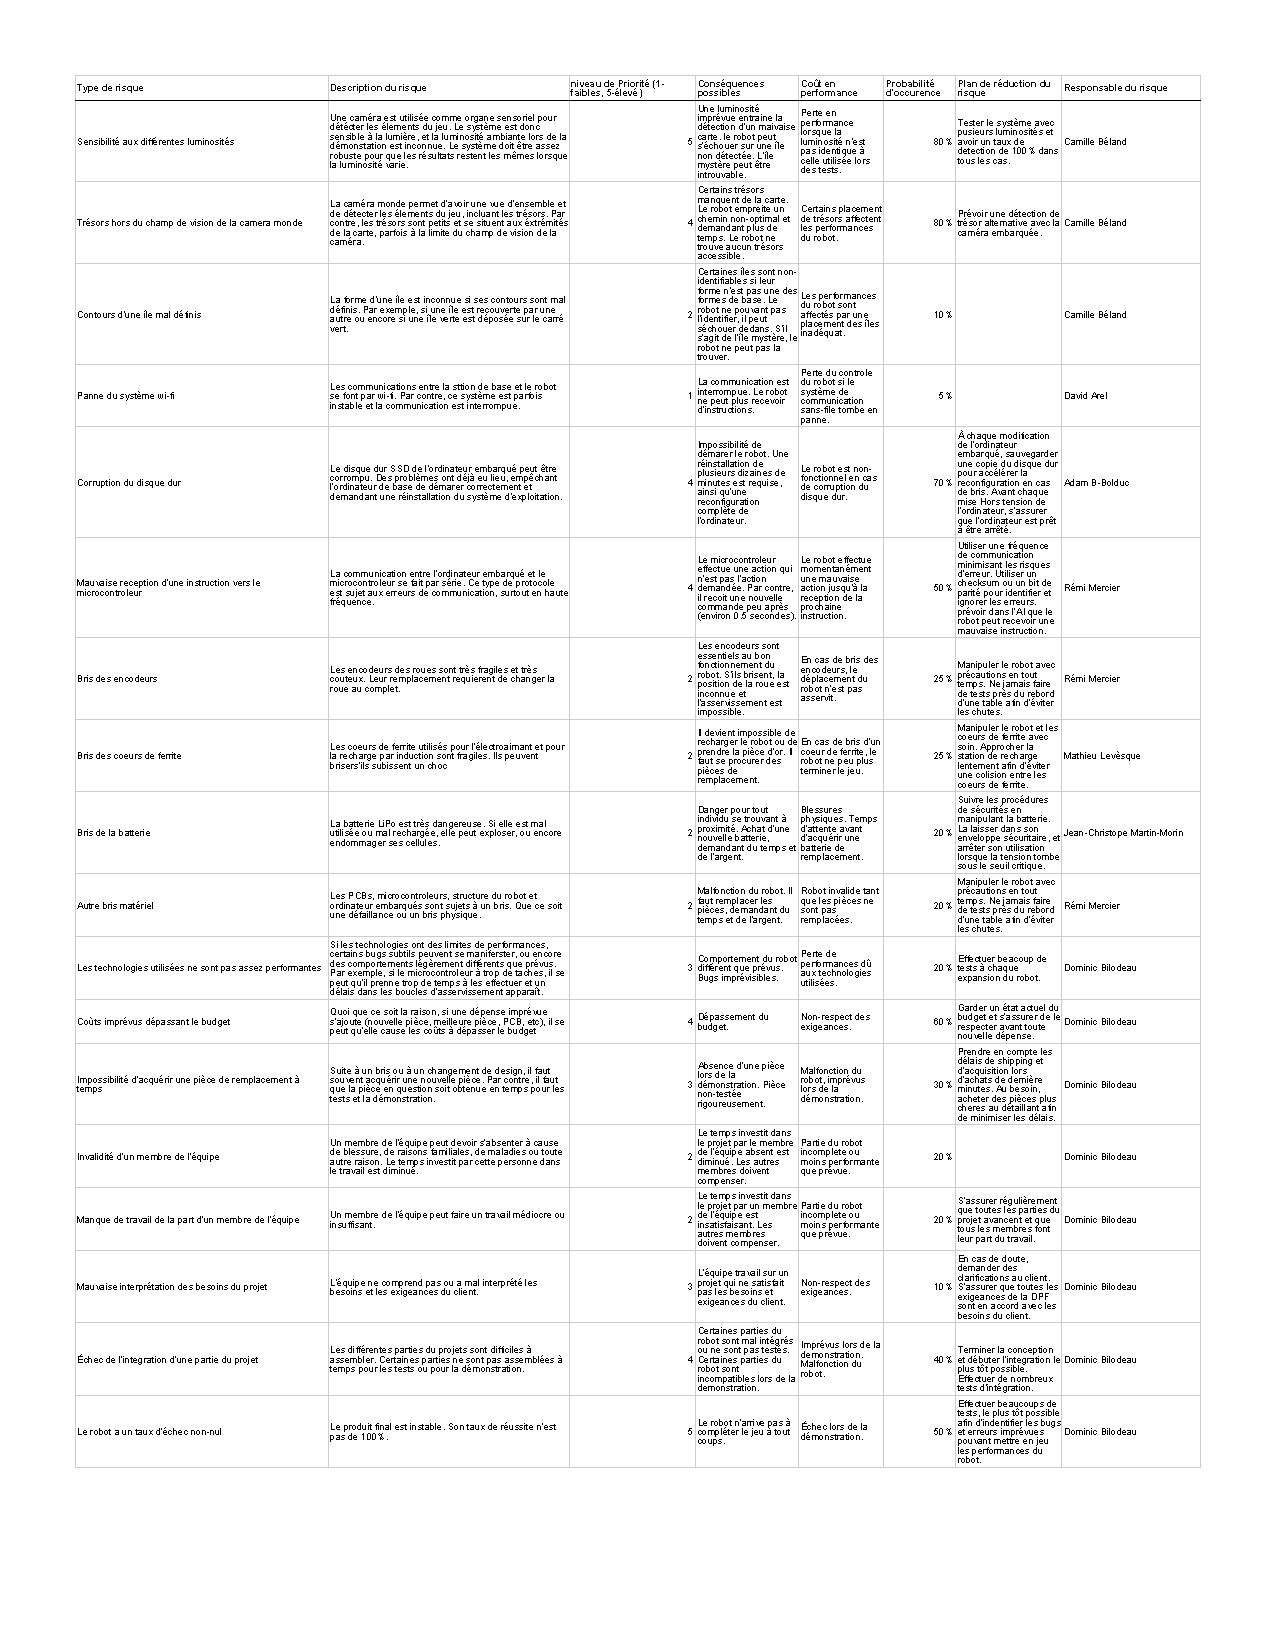
\includegraphics[scale=0.80, angle=0]{resources/risques.pdf}
\end{figure}
